\tp{Nature d'un mouvement}

\vspace*{\stretch{2}}

La trajectoire donn�e ci-contre a �t� enregistr�e � l'aide d'un palet
autoporteur lanc� sur une table inclin�e d'un angle $\beta = 45�$ par
rapport � l'horizontale. L'�tincelle �lectrique permettant le marquage
de la position du centre d'inertie du mobile a lieu toutes les $\tau =
200~ms$.

\vspace*{\stretch{2}}

\begin{enumerate}
\item Tracer la courbe passant par l'ensemble des points. Quelle est
sa nature ? Num�roter les points de $M_0$ � $M_{13}$.

\vspace*{\stretch{1}}

\item En consid�rant que $\arc{M_iM_{i+1}} = M_iM_{i+1}$, d�terminer
la vitesse instantan�e $V_1$ en $cm.s^{-1}$. Tracer le vecteur vitesse
$\vect{V_1}$. On adoptera l'�chelle $1~cm \equivalent 3~cm.s^{-1}$. Donner les
4 caract�ristiques de ce vecteur.


% symbole �quivalent <=>

\vspace*{\stretch{1}}

\item De la m�me mani�re, tracer $\vect{V_3}$, $\vect{V_5}$,
$\vect{V_7}$, $\vect{V_9}$, $\vect{V_{11}}$.

\vspace*{\stretch{1}}

\item En projetant les diff�rents vecteurs sur l'axe des abscisses et
ordonn�es, donner la valeur de leurs composantes $V_x$, $V_y$
respectives.

$\vect{V_1} = \vvectplan{V_{1x}}{V_{1y}}$
\hspace{\stretch{1}} ; \hspace{\stretch{1}}
$\vect{V_3} = \vvectplan{V_{3x}}{V_{3y}}$
\hspace{\stretch{1}} ; \hspace{\stretch{1}}
$\vect{V_5} = \vvectplan{V_{5x}}{V_{5y}}$
\hspace{\stretch{1}} ; \hspace{\stretch{1}}
... \hspace{\stretch{1}}

% to do

\vspace*{\stretch{1}}

\item Comparer les valeurs de $V_{1x}$, $V_{3x}$, $V_{5x}$, $V_{7x}$,
$V_{9x}$, $V_{11x}$ puis celles de $V_{1y}$, $V_{3y}$, $V_{5y}$,
$V_{7y}$, $V_{9y}$, $V_{11y}$. Donner la nature du mouvement du
palet. Qu'en est-il r�ellement si l'on d�compose le mouvement en sa
projection sur les axes $x$ et $y$ ?

\vspace*{\stretch{1}}

\item Rappeler le principe de l'inertie vu en seconde.

\vspace*{\stretch{1}}

\item Que peut-on dire des forces qui s'exercent sur le palet ?

\vspace*{\stretch{1}}

\item La masse du mobile utilis� est de $150~g$. \'Etablir l'inventaire
des forces en consid�rant que les frottements du palet sur la table
sont nuls. Donner les caract�ristiques de ces forces.

\vspace*{\stretch{1}}

\item Sur un sch�ma, les repr�senter en ayant pris soin de choisir une �chelle appropri�e.

\vspace*{\stretch{1}}

\item Se compensent-elles ? \`A quelle condition sur l'angle $\beta$
se compenseraient-elles ? Dans ces conditions, quelle aurait �t� la
trajectoire du mobile lanc� avec la m�me vitesse initiale $V_0$.


\end{enumerate}

\vspace*{\stretch{1}}

\newpage


\vressort{1}

\begin{center}
\begin{figure}[H]
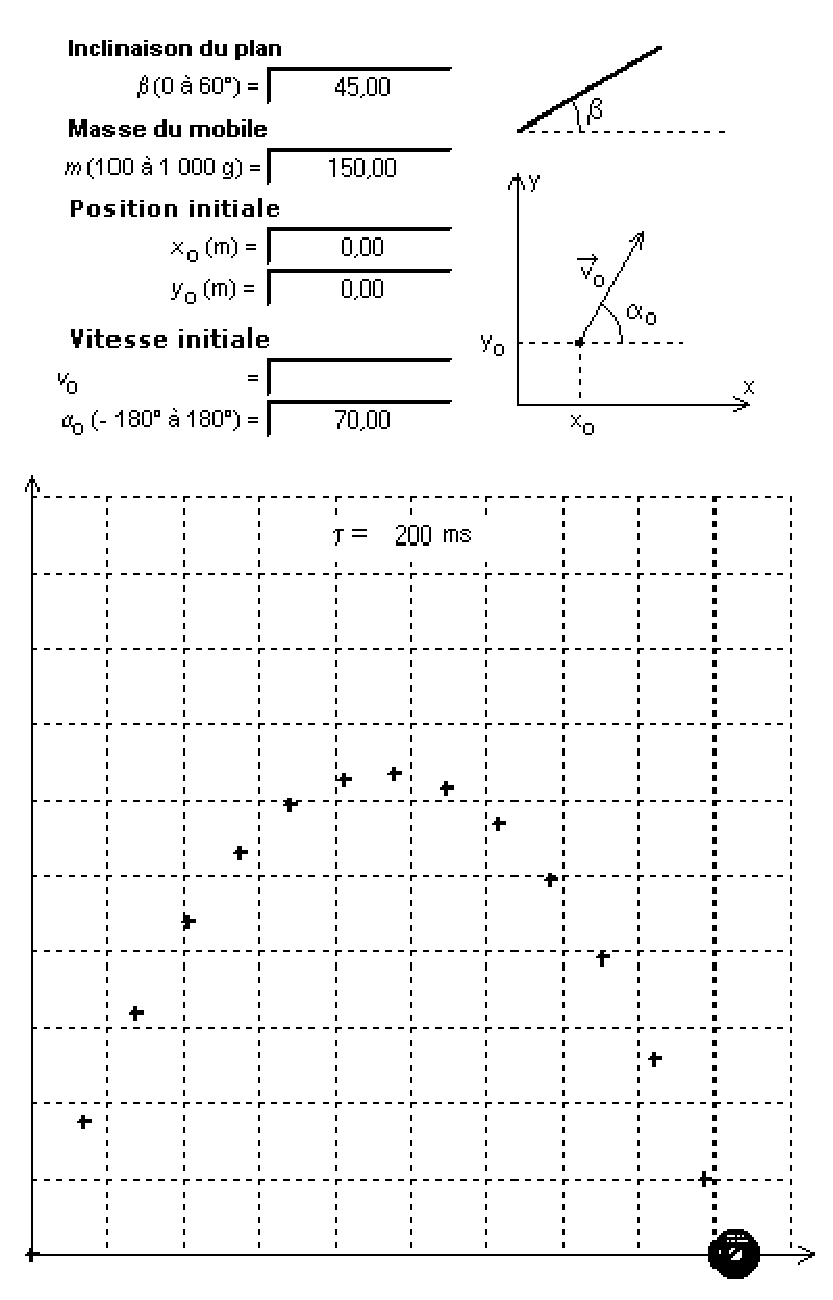
\includegraphics[width=15cm]{tp_prem_s_phys/tp04_mvt_parabolique/tp_mvt_parabo.gif.eps}
\caption{Simulation du lancer d'une balle de golf avec le logiciel
  Microm�ga \premiere S}
\end{figure}
\end{center}


\vressort{1}


% TO DO


% tau = 200~ms
% beta = 45
% m = 150~g = 0,150~kg
% x_0 = 0
% y_0 = 0
% v0 = ?
% alpha_0 = 70�




% \emph{Inclinaison du plan}\\
% \hspace{2cm}$\beta \in [0 ; 60�]$


% \vspace*{\stretch{1}}


% \emph{Masse du mobile}\\
% \hspace{2cm}$m \in [0,1 ; 1~kg]$


% \vspace*{\stretch{1}}


% \emph{Position initiale}\\
% \hspace{2cm}$x_0$ ($m$)\\
% \hspace{2cm}$y_0$ ($m$)


% \vspace*{\stretch{1}}


% \emph{Vitesse initiale}\\
% \hspace{2cm}$v_0$ ($m.s^{-1}$)\\
% \hspace{2cm}$\alpha_0 \in [-180� ; 180�]$


% \vspace*{\stretch{3}}
